
%------------------------------------------------------------------------
%
%    Copyright (C) 1985-2020  Georg Umgiesser
%
%    This file is part of SHYFEM.
%
%    SHYFEM is free software: you can redistribute it and/or modify
%    it under the terms of the GNU General Public License as published by
%    the Free Software Foundation, either version 3 of the License, or
%    (at your option) any later version.
%
%    SHYFEM is distributed in the hope that it will be useful,
%    but WITHOUT ANY WARRANTY; without even the implied warranty of
%    MERCHANTABILITY or FITNESS FOR A PARTICULAR PURPOSE. See the
%    GNU General Public License for more details.
%
%    You should have received a copy of the GNU General Public License
%    along with SHYFEM. Please see the file COPYING in the main directory.
%    If not, see <http://www.gnu.org/licenses/>.
%
%    Contributions to this file can be found below in the revision log.
%
%------------------------------------------------------------------------
\label{preprocessing}

Before you can start using the model you have to create a numerical grid.
Creating a grid is more difficult for models that work on unstructured grids
(like finite element models) than for finite difference models, where
often it is enough to have a regular gridded bathymetry to start running
simulations.

\begin{figure}[htbp]
\centering
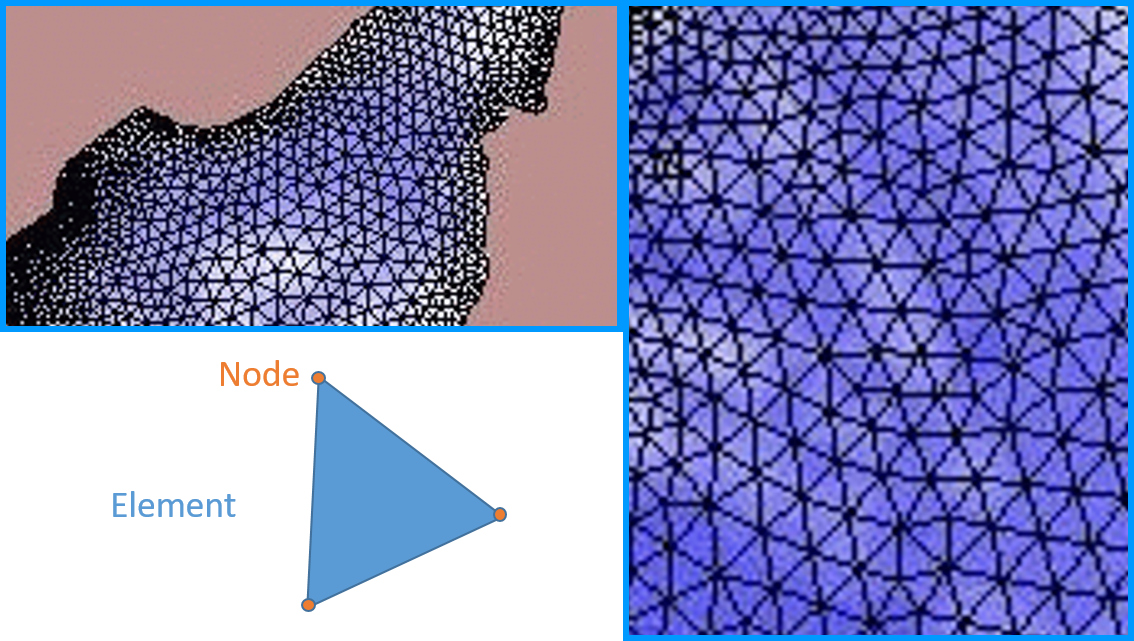
\includegraphics[scale=0.5]{example_finite_elements.png}
\caption{Example of  a finite element grid. Zoom on elements. Vertices are called nodes.}
\label{grd_example}
\end{figure}

the SHYFEM finite element grids are composed of triangular elements, 
where the vertices are called nodes. For a thorough description of the 
approach used with staggered finite elements
over such a grid refer to Appendix A.2.

This chapter describes the steps needed to create a numerical grid for SHYFEM.

The files containing the informations on the computational grid, used by SHYFEM, are two:

\begin{itemize}
\item |filename.grd| formatted
\item |filename.bas| unformatted
\end{itemize}

You must create the first one, while the second can be obtained automatically by
the first. The |bas| file is the one really used by the model.

The |grd| file can be composed of 3 different parts, describing different geometric
objects, which are: Nodes, Elements, Lines. These parts are the following:

\begin{itemize}
\item Node section, containing the nodes information and coordinates
\item Element section, containing the elements information and the their nodes
\item Line section, containing the domain contour infomation and nodes
\end{itemize}

The presence of these structures depends on type of |grd| file, for example,
in a boundary line the structures will be the line and its nodes.
For more details on the format, please, refer to |grd| file appendix~\ref{grid}.

The steps to create a |grd| file are the following and they will be described below:

\begin{enumerate}

\item obtain raw digital data of the coastline and the bathymetry and
  convert them into a |grd| format

\item smooth and reduce the coastline if needed

\item create the numerical grid with a mesh generator

\item regularize the grid

\item interpolate bathymetry onto the created grid

\item create the unformatted |bas| file

\end{enumerate}

These steps are described in the following sections.
